% Metódy inžinierskej práce

\documentclass[10pt,slovak,a4paper]{article}

\usepackage[slovak]{babel}
\usepackage[IL2]{fontenc} 
\usepackage[utf8]{inputenc}
\usepackage{graphicx}
\usepackage{url} 
\usepackage{hyperref} 
\usepackage{booktabs}
\usepackage{multirow}
\usepackage{cite}

\pagestyle{headings}

\title{Google Classroom,  MS Teams a ich využitie vo výučbe.\thanks{Semestrálny projekt v predmete Metódy inžinierskej práce, ak. rok 2020/21, vedenie: Ing. Michal Hatala, PhD. }}

\author{Filip Cák\\[2pt]
	{\small Slovenská technická univerzita v Bratislave}\\
	{\small Fakulta informatiky a informačných technológií}\\
	{\small \texttt{xcak@stuba.sk}}
	}

\date{\small 8. november 2020}



\begin{document}

\maketitle

\begin{abstract}
V mojom projekte sa plánujem zamerať na výhody a efektivitu využitia online platforiem Google Classroom a MS Teams pri výučbe a zároveň porovnať tieto dve služby. Počas pandémie boli školy nútené nájsť alternatívu prezenčného vzdelávania. Mnohé si vybrali práve jednu z týchto 2 alternatív. \cite {COVID-19clanok} V mojom projekte by som chcel bližšie opísať možnosti online vzdelávania cez Google Classroom alebo MS Teams \cite {porovnanie}, ktoré mohli byť zavedené aj skôr, ako výpomoc pri komunikácii medzi žiakmi a učiteľmi. Zámerom je vyhodnotiť ako by to obom stranám uľahčilo komunikáciu, prehľadnosť zadaných úloh a cvičení ako aj následnú kontrolu. Poukázať aj na možný priestor zlepšenia spolupráce na tímových projektoch.
\end{abstract}



\section{Úvod}
Pandémia spôsobená vírusom COVID-19 sa začala ešte na jar 2020 a zasiahla mnohé časti spoločnosti, okrem iného aj školstvo. Školy stredné aj vysoké boli nútené zrušiť prezenčné vyučovanie a museli nájsť náhradu. Mnoho škôl na Slovensku reagovalo promptne a začali vyučovať dištančne v online forme. Postupne sa pridávali ďalšie školy, ktoré skúšali rôzne platformy, cez ktoré by mohli vyučovať. Napríklad Microsoft Teams, Google Classroom, Webex, Zoom. [3] V mojom projekte budem opisovať možné benefity Google Classrom a Microsoft Teams a ich využívania aj počas prezenčného vyučovania. 

\section{Google Classroom} \label{Google Classroom}

Google Classroom bol sprístupnený verejnosti už v roku 2014. \cite {release_date} Táto e-learningová platforma sa najskôr využívala na lepšiu komunikáciu medzi učiteľmi a žiakmi a na vyššiu efektivitu - Google Docs na zápis poznámok, Drive na zdieľanie dokumentov a Gmail na komunikáciu. Postupne medzi tieto aplikácie pridali aj Google Sheets, Google Slides, Google Calendar, Google Jamboard a podobne. V roku 2020 integrovali aj službu Google Meet, kde umožňujú učiteľom mať ku každej triede jedinečný link na videohovor. Google Classroom je prístupný cez webové prehliadače rovnako ako aj cez aplikácie na Chrome OS, iOS a Androide. Kedže ponúka všetky tieto možnosti, stáva sa ľahko prístupným a umožnuje to hocikomu používať. \cite {COVID-19clanok} Učitelia majú možnosť si tam ukladať všetky svoje práce rovnako ako aj žiaci. Do triedy je možné nahrať aj video ako z pohľadu učiteľa tak aj študenta. Študent má vo svojom rozhraní intuitívne vyobrazené miesta, kam odovzdáva svoju prácu. Tú mu vie učiteľ jednoducho opraviť. V nasledujúcom odseku bližšie opíšem niektoré benefity.

\subsection{Model Google Classroom platformy} \label{Google Classroom: Google Classroom platforma}

\begin{itemize}
	\item Admin môže hromadne vytvoriť mailové adresy pre študentov a následne im posielať kolektívne maily podľa jednotlivých podtried. 
	\item Odovzdané súbory automaticky zmenia názov podľa mien študentov a sú uložené do jedného priečinku.
	\item Jednoduchý prístup cez aplikáciu alebo prehliadač.
	\item Viac žiakov má možnosť spolupracovať v jednom súbore.
	\item Zadarmo -
Google Classroom je momentálne zadarmo pre školy aj pre žiakov. Nevyžaduje mať založený mail v Gmaili. Ak by chcel človek využívať nástroje ako Docs, Sheets, a podobne, no zároveň nie je šudentom školy, ktorá využíva Google Classroom, je potrebné mať založený účet v Gmaili. 
	\item Úspora času - softvérový inžinier Google Classroom poznamenal, že vytvorili triedu kde, sa dá šetriť s časom. Zmienil hlavne rýchlu dostupnosť učiva pre celú triedu, ako aj uľahčenie prístupu učiteľa k odovzdaným prácam a export známok do Google Sheets, čo urobí značne prehľadnejším čítať dáta. \cite {GoogleClassroomPBL}
	\end{itemize}


\section{MS Teams} \label{MS Teams}
Spoločnosť Microsoft zverejnila príchod platformy MS TEAMS v roku 2016, ktorá bola postupne rozvýjaná a momentálne je súčasťou balíka Office 365. Postupne nahrádza aplikáciu Skype for Business, tá vznikla premenovaním aplikácie Lync a pridaním podpory pre videohovory so Skype užívateľmi. Koniec fungovania Skype for Business je ohlásený na 31 júla 2021. \cite{ohlasene_ukoncenie} TEAMS prináša nové možnosti komunikácie, ale aj efektívne vytváranie a zdieľanie súborov. Táto platforma je zameraná nielen pre školy rôznych stupňov a triedy v nich, ale aj ako je v názve uvedené - pre tímy. Funkcionality sú upravené tak, aby vyhovovali aj pre komunikáciu vo väčších tímoch alebo firmách. MS TEAMS je prístupný ako aplikácia na Windows, macOS, Linux, Android aj iOS, ale dá sa spustiť aj vo webovom prehliadači. Táto platforma je voľne dostupná a užívateľsky prívetivá. \cite {MS-TEAMS}

\subsection{Model MS TEAMS platformy} \label{MS TEAMS: MS TEAMS platforma}

\begin{itemize}
	\item Študent potrebuje mať vytvorené konto v Microsofte, do triedy sa pripojí pomocou url linku poskytnutého adminom.
	\item Dostupnosť offline - pripojenie na internet nie je potrebné pre prístup k OneDrive, OneNote, Class Notebook. Súbory sa synchronizujú.
 	\item Ak učiteľ dovolí - študent môže aj po odovzdaní upraviť svoju prácu, zmeny sú zaznamenané.
	\item Jednoduchý prístup cez aplikáciu alebo prehliadač.
	\item Kompaktibilné s 3 najväčšími platformami - PC, Android, iOS - samostaná aplikácia pre každú platfomu. 
\cite {porovnanie}
	\end{itemize}


\section{Rozdiely } \label{Rozdiely}
Každá škola má svoje špecifické požiadavky pre systém na výučbu. Google Classroom aj MS TEAMS sú momentálne lídry v zlepšení online alebo aj offline vyučovania. Obe platformy sú si pomerne podobné. V nasledujúcich bodoch prinášam pár hlavných rozdielov medzi nimi:\cite{porovnanie}


\begin{itemize}
	\item Limit študentov v jednej triede je 250 pre Google Classroom.  Do tímu v MS TEAMS sa môže pripojiť viac ľudí, no prideľovanie úloh nie je podporované pri viac ako 200 študentoch.
	\item Google Classroom automaticky premenuje súbor tak, aby názov obsahoval meno šudenta.
	\item Po synchronizácii súborov MS TEAMS nevyžaduje pripojenie na internet pre prácu s nimi.	
	\item MS TEAMS platforma je dostupná pre PC, Android aj iOS vo forme aplikácie, ale dá sa spustiť aj cez webový prehliadač. Google Classroom nie je prístupný vo forme aplikácie pre PC.
	\item Google Classrom umožnuje študentovi zrušiť odovzdanie súboru a nahrať nový. Ako aj viacnásobné upravenie súboru po vrátení od učiteľa. Zmeny sa ukladajú. Pri MS TEAMS študent môže upraviť svoj odovzdaný súbor až keď mu ho učiteľ vráti. Tento úkon býva označený ako - naspäť v rukách.
	\item Vysvetlenie hodnotenia jednotlivých častí úlohy je implementované pri MS TEAMS. V Google Classroom iba s použitím externého rozšírenia.
	\item MS TEAMS umožnuje učiteľom pozerať odovzdané súbory iba na počítači.
\end{itemize}

\section{Pohľad študenta} \label{pohľad studenta}
Pri vypracovávaní môjho projektu som vytvoril dotazník. Študenti v ňom vyjadrili svoj názor na jednotlivé platformy, ktoré využívajú pri vyučovaní na školách. Dotazník vyplnilo 77 študentov stredných a vysokých škôl. Vyhodnotil som údaje, ktoré obsahovali informácie o platformách, ktorým je venovaný tento článok. Výsledky sú nasledovné. Google Classroom by odporučilo 89,5\% opýtaných študentov, ktorí ho využívajú pri výučbe. Tabuľka \ref{tab:tabulkaGoogle}. Zároveň väčšina sa tam vie veľmi dobre zorientovať Obrázok \ref{diagramGoogle}. MS TEAMS by odporučilo 82,7\% opýtaných študentov, ktorí ho využívajú pri výučbe. Tabuľka \ref{tab:tabulkaMS}. Zároveň väčšina sa tam vie dobre zorientovať, no táto platforma podľa opýtaných študentov nie je až tak prehľadná.  Obrázok \ref{diagramMS}.


% Table generated by Excel2LaTeX from sheet 'Google Classroom'
\begin{table}[htbp]
  \centering
  \caption{Študenti využívajúci Google Classroom}
    \begin{tabular}{|l|cc|r|}
    \toprule
    \multicolumn{4}{|c|}{\multirow{2}[2]{*}{Odporučil by si niekomu Google Classroom ako platformu dobré online vyučovanie?}} \\
    \multicolumn{4}{|c|}{} \\
    \midrule
    ÁNO   & \multicolumn{2}{c|}{17 študentov} & 89,5\% \\
    \midrule
    NIE   & \multicolumn{2}{c|}{2 študenti} & 10,5\% \\
    \bottomrule
    \end{tabular}%
  \label{tab:tabulkaGoogle}%
\end{table}%


% Table generated by Excel2LaTeX from sheet 'MS TEAMS'
\begin{table}[htbp]
  \centering
  \caption{Študenti využívajúci MS TEAMS}
    \begin{tabular}{|l|cc|r|}
    \toprule
    \multicolumn{4}{|c|}{\multirow{2}[2]{*}{Odporučil by si niekomu MS TEAMS ako platformu dobré online vyučovanie?}} \\
    \multicolumn{4}{|c|}{} \\
    \midrule
    ÁNO   & \multicolumn{2}{c|}{43 študentov} & 82,7\% \\
    \midrule
    NIE   & \multicolumn{2}{c|}{9 študentov} & 17,3\% \\
    \bottomrule
    \end{tabular}%
  \label{tab:tabulkaMS}%
\end{table}%


\paragraph{Grafické vyjadrenie informácií v informatike} \label{Grafické vyjadrenie informácií v informatike} - prehľadné znázornenie údajov, s ktorými sa pracuje v projekte alebo článku je veľmi užitočné. Človek si skôr zapamätá údaje ak ich vidí graficky zobrazené, napríklad vo forme grafu.

\paragraph{Bibliografia a citovanie v technickom texte} \label{Bibliografia a citovanie v technickom texte} - vždy je potrebné vo svojej práci uviesť bibliografický odkaz na článok alebo knihu ak sú údaje z nej zahrnuté v projekte. Čitateľ tak dostane možnosť si overiť odkiaľ autor čerpal informácie pri písaní článku.

\paragraph{Inžinierska práca v informatike a písanie technického textu}\label{Inžinierska práca v informatike a písanie technického textu} - inžinier vyvíja metódy. To čo vypracuje potrebuje dostatočne opísať a tým vzniká dokumentácia. Tá by mala byť prehľadná a delená na jednotlivé sekcie.


\section{Záver} \label{zaver} 
MS TEAMS spoločne s balíkom Ofiice rovnako ako aj Google Classroom s aplikáciami Docs, Sheets, Jamboard a ďalšími vedia dostatočne zabezpečiť dištančnú výučbu pre školy. Študentom tam môžu byť pridelované úlohy, následne aj ohodnotené. Obe platformy sú vhodné pre lepšie zvládnutie dištančného vzdelávania. Majú viaceré veľmi dobré funkcionality, ktoré boli spomenuté v častiach ~\ref {Google Classroom: Google Classroom platforma}  a  ~\ref{MS TEAMS: MS TEAMS platforma}. Tieto prednosti robia Google Classroom aj MS TEAMS dobrými nástrojmi aj pre prezenčnú výučbu. V oboch prípadoch sú platformy prevažne prehľadné a mimoriadne ľahko dostupné. Vedelo by to preto zlepšiť prístup študentov k zadaným materiálom. Spolupráca viacerých užívateľov na jednom súbore môže byť veľmi benefičná pre zlepšenie tímovej práce v triedach. Celkovo si myslím, Google Classroom aj MS TEAMS v nasledujúcich rokoch zmenia výučbu na školách.

\begin {figure}
\begin {center}
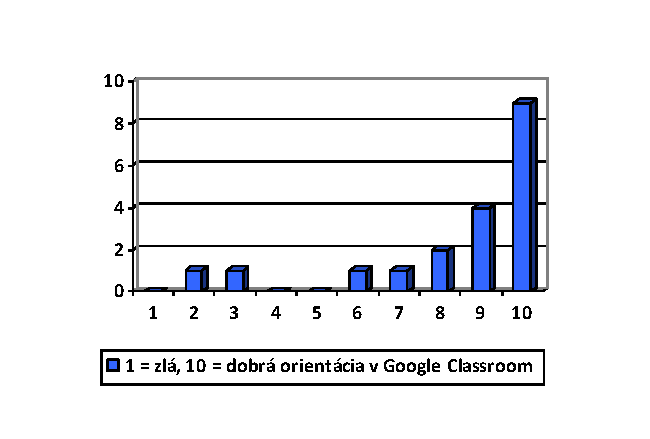
\includegraphics[scale=1]{diagramGoogle.pdf}
\caption{Študenti využívajúci Google Classroom}
\label {diagramGoogle}
\end {center}
\end{figure}


\begin {figure}
\begin {center}
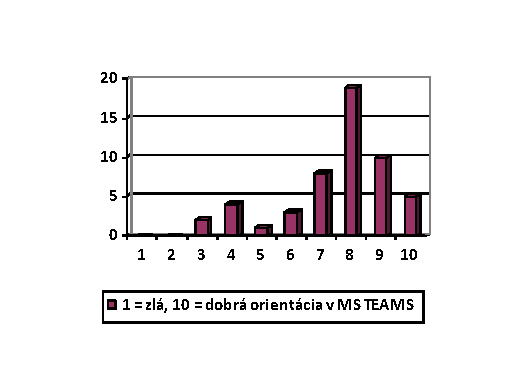
\includegraphics[scale=1.25]{diagramMS.pdf}
\caption{Študenti využívajúci MS TEAMS}
\label {diagramMS}
\end {center}
\end{figure}

\bibliography{literatura_cak}
\bibliographystyle{unsrt}
\end{document}
